% Path: docs/report_final_it.tex
\documentclass[11pt,a4paper]{article}

\usepackage[utf8]{inputenc}
\usepackage[T1]{fontenc}
\usepackage[italian]{babel}
\usepackage{geometry}
\usepackage{booktabs}
\usepackage{graphicx}
\usepackage{float}
\usepackage{hyperref}
\usepackage{enumitem}
\usepackage{setspace}

\geometry{margin=1in}
\onehalfspacing

\title{Image\_Captioning\_CNN\_LSTM}
\author{Giuseppe Dimonte \\ Matricola 367431}
\date{Anno Accademico 2025/26}

\begin{document}

\begin{titlepage}
\centering
{\Large Università degli Studi di Parma \par}
\vspace{0.3cm}
{\large Dipartimento di Ingegneria e Architettura \par}
\vspace{0.3cm}
{\large Corso di Laurea in Ingegneria Informatica \par}
{\large Curriculum: Intelligenza Artificiale \par}
\vspace{1.2cm}
{\Large \textbf{Deep Learning e Modelli Generativi} \par}
\vspace{0.5cm}
{\large Docente: Prof. Andrea Prati \par}
\vspace{1.5cm}
{\huge \textbf{Image\_Captioning\_CNN\_LSTM} \par}
\vspace{1.5cm}
{\large \textbf{Studente:} Giuseppe Dimonte \par}
{\large \textbf{Matricola:} 367431 \par}
{\large \textbf{Email:} giuseppe.dimonte@studenti.unipr.it \par}
\vfill
{\large Anno Accademico 2025/26 \par}
\end{titlepage}

\tableofcontents
\newpage

\begin{abstract}
Questo report presenta l'implementazione e la valutazione di un sistema di image captioning basato su architettura CNN-LSTM addestrato sul dataset Flickr8k. Il progetto copre l'intera pipeline richiesta dall'assegnamento: preprocessing delle caption, costruzione del vocabolario, preparazione dei file di training e validation, addestramento supervisionato, valutazione con metriche BLEU e analisi qualitativa dei risultati. È stata inoltre condotta una campagna sperimentale controllata su quattro configurazioni: baseline, rimozione dello scheduled sampling, rimozione del label smoothing e fine-tuning della CNN. Il miglior risultato è stato ottenuto dalla configurazione con fine-tuning, che ha raggiunto un BLEU-4 pari a 0.0649, superiore al valore di baseline pari a 0.0472.
\end{abstract}

\section{Introduzione}

L'image captioning è un problema multimodale in cui un sistema deve ricevere un'immagine in input e generare una descrizione testuale coerente con il contenuto visivo. Il compito combina due aspetti distinti: comprensione visiva e generazione linguistica. Per questo motivo può essere formulato naturalmente come problema image-to-sequence.

L'obiettivo di questo progetto è stato implementare una pipeline completa di image captioning basata su CNN-LSTM, in accordo con i requisiti dell'assegnamento del corso. Oltre alla realizzazione del modello, il lavoro ha richiesto una particolare attenzione alla riproducibilità dell'intero flusso, dalla preparazione dei dati alla raccolta sistematica dei risultati sperimentali.

\section{Traccia dell'assegnamento}

La traccia richiedeva:
\begin{itemize}[leftmargin=*]
    \item l'utilizzo del dataset Flickr8k;
    \item l'implementazione di una architettura CNN-LSTM;
    \item la pulizia del testo delle caption;
    \item la costruzione di un dizionario/vocabolario da salvare su file;
    \item l'accoppiamento tra feature visuali e sequenze testuali durante il training;
    \item la generazione delle caption in fase di test a partire dall'output del decoder.
\end{itemize}

Il progetto finale soddisfa questi requisiti attraverso una pipeline modulare e riproducibile.

\section{Dataset e preprocessing}

\subsection{Dataset Flickr8k}

Flickr8k è un dataset di image captioning in cui ogni immagine è associata a cinque caption di riferimento. Nel progetto sono stati prodotti artefatti preprocessati per rendere il workflow ripetibile:
\begin{itemize}[leftmargin=*]
    \item \texttt{data/vocab.json}
    \item \texttt{data/Flickr8k\_text/train.csv}
    \item \texttt{data/Flickr8k\_text/val.csv}
    \item \texttt{data/Flickr8k\_text/test\_captions.json}
\end{itemize}

Dimensioni finali osservate:
\begin{itemize}[leftmargin=*]
    \item 30000 righe di training
    \item 5000 righe di validation
    \item 1000 immagini di test
    \item 5 caption di riferimento per immagine
\end{itemize}

\subsection{Pulizia del testo}

Le caption sono state preprocessate applicando:
\begin{itemize}[leftmargin=*]
    \item conversione in minuscolo
    \item rimozione della punteggiatura
    \item rimozione dei numeri
    \item rimozione delle parole costituite da una sola lettera
    \item normalizzazione degli spazi
\end{itemize}

Il vocabolario finale contiene 2985 token, inclusi i token speciali \texttt{<pad>}, \texttt{<bos>}, \texttt{<eos>} e \texttt{<unk>}.

\section{Architettura del modello}

Il sistema implementato segue una struttura encoder-decoder.

\subsection{Encoder}

L'encoder utilizza InceptionV3 pre-addestrata su ImageNet. Il layer finale di classificazione è stato rimosso e le feature estratte sono state proiettate nello spazio di embedding utilizzato dal decoder.

\subsection{Decoder}

Il decoder è una LSTM a singolo layer. Durante il training riceve in input la rappresentazione dell'immagine e la sequenza di token della caption. Un layer lineare finale mappa gli hidden state del decoder nello spazio del vocabolario per la predizione del token successivo.

\subsection{Tecniche di training}

Il codice supporta:
\begin{itemize}[leftmargin=*]
    \item scheduled sampling
    \item label smoothing
    \item gradient clipping
    \item checkpointing del modello
    \item resume da checkpoint
    \item valutazione BLEU-1/BLEU-2/BLEU-3/BLEU-4
\end{itemize}

\section{Dettagli implementativi}

La repository è organizzata in moduli distinti:
\begin{itemize}[leftmargin=*]
    \item \texttt{src/vocab\_builder.py}: pulizia testo, costruzione vocabolario, esportazione split
    \item \texttt{src/prepare\_data.py}: script rapido per la preparazione dei dati
    \item \texttt{src/dataset.py}: dataset e batching
    \item \texttt{src/model.py}: definizione della CNN-LSTM
    \item \texttt{src/train.py}: training loop e checkpoint
    \item \texttt{src/eval.py}: generazione caption e calcolo BLEU
    \item \texttt{src/visualize.py}: figure qualitative
    \item \texttt{src/ui\_streamlit.py}: demo interattiva opzionale
\end{itemize}

Durante la revisione del progetto sono stati corretti diversi problemi strutturali, tra cui:
\begin{itemize}[leftmargin=*]
    \item parsing scorretto del formato Flickr8k
    \item allineamento della loss sul next-token prediction
    \item attivazione reale del fine-tuning dell'encoder
    \item generazione automatica degli artefatti mancanti
\end{itemize}

\section{Setup sperimentale}

Tutti gli esperimenti finali sono stati eseguiti su:
\begin{itemize}[leftmargin=*]
    \item ambiente Python: \texttt{captioning}
    \item PyTorch: \texttt{2.9.1+cpu}
    \item device: CPU
\end{itemize}

Configurazioni confrontate:
\begin{enumerate}[leftmargin=*]
    \item Baseline
    \item No Scheduled Sampling
    \item No Label Smoothing
    \item Fine-tuning della CNN
\end{enumerate}

Nella comparazione finale tutte le configurazioni sono state eseguite per 5 epoche.

\section{Risultati quantitativi}

\begin{table}[H]
\centering
\caption{Confronto BLEU tra gli esperimenti finali.}
\begin{tabular}{lcccc}
\toprule
Esperimento & BLEU-1 & BLEU-2 & BLEU-3 & BLEU-4 \\
\midrule
Baseline & 0.2553 & 0.1556 & 0.0928 & 0.0472 \\
No Scheduled Sampling & 0.2232 & 0.1242 & 0.0717 & 0.0396 \\
No Label Smoothing & 0.2404 & 0.1435 & 0.0809 & 0.0394 \\
Fine-tuning & 0.3301 & 0.2022 & 0.1189 & 0.0649 \\
\bottomrule
\end{tabular}
\end{table}

\begin{table}[H]
\centering
\caption{Riassunto del training.}
\begin{tabular}{lccc}
\toprule
Esperimento & Best Val Loss & Final Train Loss & Final Val Loss \\
\midrule
Baseline & 4.1927 & 4.8016 & 4.2332 \\
No Scheduled Sampling & 4.0106 & 3.5373 & 4.0234 \\
No Label Smoothing & 3.5029 & 4.0860 & 3.5738 \\
Fine-tuning & 3.6614 & 4.7512 & 4.2861 \\
\bottomrule
\end{tabular}
\end{table}

\section{Discussione dei risultati}

La baseline fornisce il punto di riferimento del progetto. Rimuovendo lo scheduled sampling si osserva un peggioramento di tutte le metriche BLEU, anche se la training loss risulta inferiore. Questo suggerisce che lo scheduled sampling migliori la generalizzazione del decoder durante la generazione autoregressiva.

Anche la rimozione del label smoothing produce un peggioramento delle metriche rispetto alla baseline, indicando che tale tecnica contribuisce positivamente alla qualità delle caption generate.

La configurazione con fine-tuning della CNN ha ottenuto i migliori risultati complessivi, migliorando il BLEU-4 da 0.0472 a 0.0649. Nel contesto di questo studio, il fine-tuning è quindi la scelta più efficace.

\section{Analisi qualitativa}

\begin{figure}[H]
    \centering
    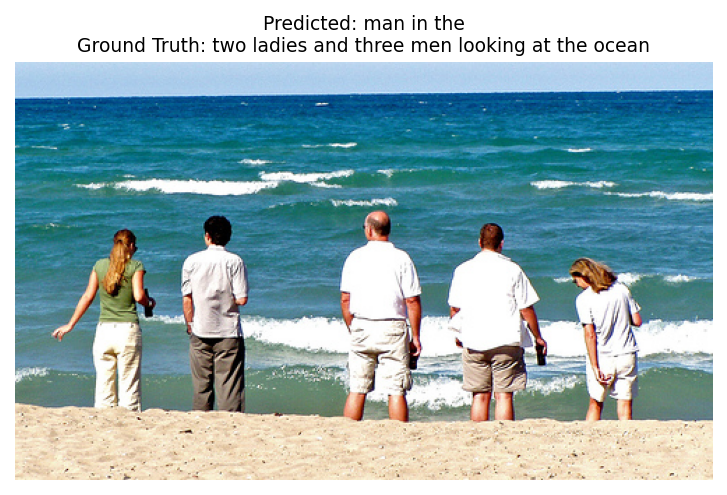
\includegraphics[width=0.8\textwidth]{selected_figures/baseline_example.png}
    \caption{Esempio qualitativo della baseline. La caption predetta è parzialmente coerente ma rimane generica e incompleta rispetto alla descrizione reale.}
    \label{fig:baseline_it}
\end{figure}

\begin{figure}[H]
    \centering
    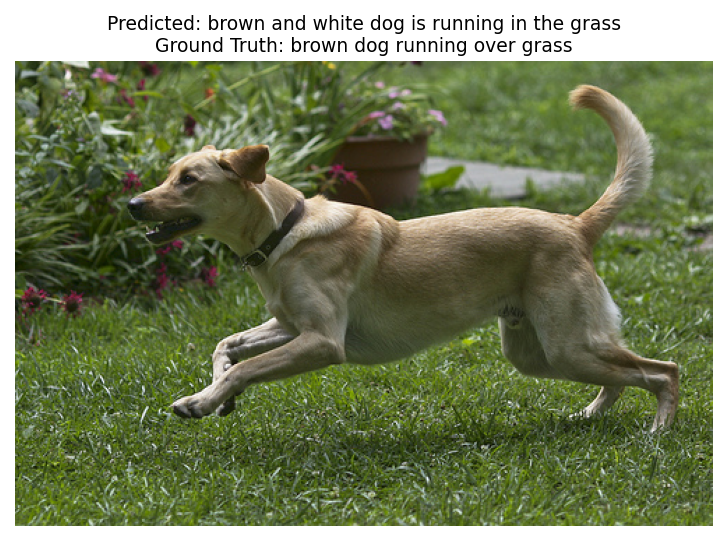
\includegraphics[width=0.8\textwidth]{selected_figures/finetune_example.png}
    \caption{Esempio qualitativo del modello fine-tuned. La caption identifica correttamente l'oggetto principale e l'azione.}
    \label{fig:finetune_it}
\end{figure}

\begin{figure}[H]
    \centering
    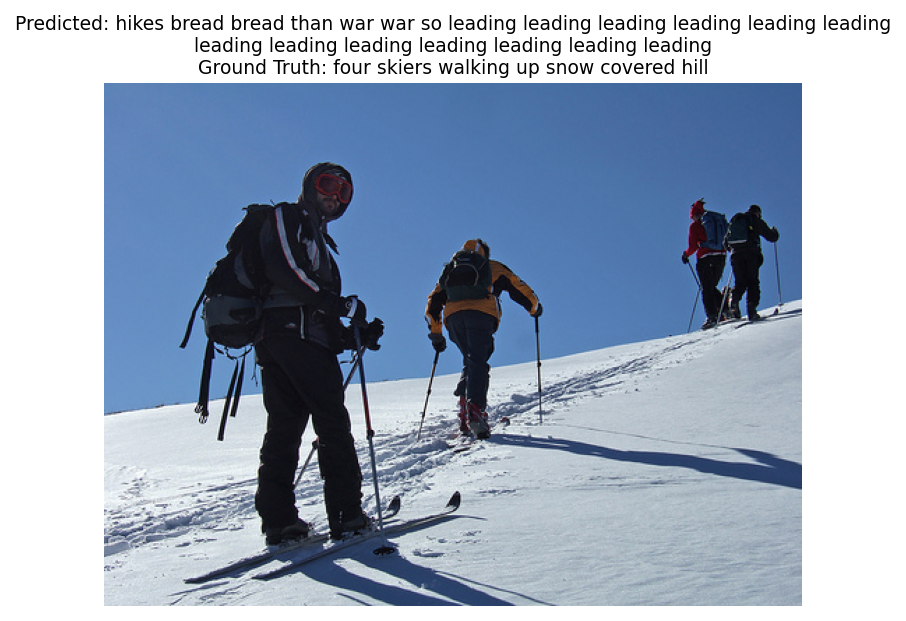
\includegraphics[width=0.8\textwidth]{selected_figures/failure_case.png}
    \caption{Failure case. L'output mostra ripetizioni e incoerenza semantica, evidenziando i limiti residui del modello.}
    \label{fig:failure_it}
\end{figure}

\section{Limiti del progetto}

\begin{itemize}[leftmargin=*]
    \item Tutti gli esperimenti sono stati eseguiti su CPU, con tempi di training elevati.
    \item Flickr8k è un dataset relativamente piccolo per image captioning.
    \item L'architettura studiata è classica e non include confronti con modelli Transformer.
\end{itemize}

\section{Conclusioni}

Il progetto ha realizzato una pipeline completa di image captioning con CNN-LSTM su Flickr8k, dalla preparazione dei dati fino alla valutazione quantitativa e qualitativa. I risultati sperimentali mostrano che scheduled sampling e label smoothing migliorano le prestazioni rispetto alle rispettive ablation, mentre il fine-tuning dell'encoder produce il miglior risultato finale. La repository contiene ora codice, log, checkpoint, figure e file di risultati sufficienti per una consegna accademica completa e riproducibile.

\section*{Artefatti disponibili}

\begin{itemize}[leftmargin=*]
    \item \texttt{results/metrics\_summary.csv}
    \item \texttt{results/experiment\_summary.csv}
    \item \texttt{results/*\_predictions.json}
    \item \texttt{logs/*}
    \item \texttt{figures/*}
    \item \texttt{LAB\_LOG.md}
\end{itemize}

\end{document}
